

\documentclass{article}[14pt, oneside, a4paper, times]

\usepackage[utf8]{inputenc}
\usepackage[english]{babel}
\usepackage[T1]{fontenc}
\usepackage{epsfig}           % para incluir figuras
\usepackage{subfig}
\usepackage{graphicx}
\usepackage{setspace}
\usepackage{vmargin}
\usepackage{algorithm}
\usepackage{algorithmic}
\usepackage{amsfonts} 
\usepackage{amssymb}


\setpapersize [portrait]{A4}
\setmarginsrb {30mm} % margem esquerda
              {10mm} % margem topo
             {30mm} % margem direita
            {20mm} % margem pé
           {2ex}  % altura do espaco para cabeçalho
           {5ex}  % espaço entre fim do cabeçalho e início do texto
          {0pt}  % altura do espaço para rodapé
         {20mm}  % espaço entre fim do texto e fim do rodapé

\doublespacing

%=======================================================================
\pagestyle{myheadings}
\begin {document}

\title{Classification using Hidden Markov Models 
\\ \large Report \#03}
\author{Luiz S. Oliveira and Marisa Morita  
\\
\vspace {-10pt}
Federal University of Parana (UFPR)\\
\vspace {-10pt}
Department of Informatics (DInf)\\
\vspace {-10pt}
R. Rua Cel. Francisco H. dos Santos, 100, Curitiba, PR, Brazil \\
lesoliveira@inf.ufpr.br \\ 
}


\date{}
\maketitle
%\vspace{-2\baselineskip}
\thispagestyle{empty}

%\begin{abstract}

%bla bla


%\end{abstract}

%%%%%%%%%%%%%%%%%%%%%%%%%%%%%%%%%%%%%%%%%%%%%%%%%%%%%%%%%%%%%%%%%%%%%%%%%%%%%%%%%
% Introduction 
%%%%%%%%%%%%%%%%%%%%%%%%%%%%%%%%%%%%%%%%%%%%%%%%%%%%%%%%%%%%%%%%%%%%%%%%%%%%%%%%%
\section{Introduction} 

This report describes the activities performed in Aug/Sep 2013, which consist in using Hidden Markov Models (HMM) to classify handwritten words using the global features introduced in the last report. In order to make this report self-contained, in Section \ref{hmm-theory:sec} we present the theory of HMMs. Then, in Section \ref{modelling:Sec} we describe how we have built the HMM models to recognise handwritten words while in Section \ref{experiments:sec} we report some experimental results. Finally, Section \ref{conclusion:sec} concludes this report pointing out our next steps. The source codes of all experiments are available in the SVN repository. 





\section{Introduction to HMM}
\label{hmm-theory:sec}

A Hidden Markov Model (HMM) is a doubly stochastic process, with an underlying
stochastic process that is not observable (hence the word hidden), but can be
observed through another stochastic process that produces the sequence of
observations \cite{Rabiner89}. The hidden process consists of a set of states
connected to each other by transitions with probabilities, while the observed
process consists of a set of outputs or observations, each of which may be
emitted by each state according to some output probability density function
(pdf). Depending on the nature of this pdf, several kinds of HMMs can be
distinguished. If the observations are naturally discrete or quantized using
vector quantization \cite{Huang90}, and drawn from an alphabet or a codebook,
the HMM is called discrete. If these observations are continuous we are dealing
with a continuous HMM, with a continuous pdf usually approximated by a mixture
of normal distributions. In the context of this thesis we consider discrete
HMMs.

In some applications, it is more convenient to produce observations by
transitions rather than by states. Furthermore, it is sometimes useful to allow
transitions with no output in order to model, for instance, the absence of an
event in a given stochastic process. If we add the possibility of using more
than one feature set to describe the observations, we must modify the classic
formal definition of HMMs \cite{Rabiner89}. These modifications can be found in
\cite{ElYacoubi99-1} and they are also described in this appendix. In this
case, the following parameters are required:

\begin{itemize}

    \item $T$: length of the observation sequence $O = \{ o_0, o_1, \ldots, o_{T-1} \}$,
        where $o_t = (o_t^0, o_t^1, \ldots, o_t^{P-1})$, the observation
        $o_t^p$ at time $t$ being drawn from the $p^{th}$ finite feature set,
        and $p = 0,1, \ldots, P-1$.

    \item $N$: number of states in the model.

    \item $M_p$: number of possible observation symbols for the $p^{th}$ feature set.

    \item $S = \{ s_0, s_1, \ldots, s_{N-1} \}$: set of possible states of the model.

    \item $Q = \{ q_t \}$: $q_t$ denotes the state at time $t$.

    \item $V_p = \{ v_0^p, v_1^p, \ldots, v_{M-1}^p \}$: codebook  or discrete set
        of possible observation symbols corresponding to the $p^{th}$ feature set.

    \item $A = \{ a_{ij} \}$, $a_{ij} = P[ q_{t+1} = s_j | q_t = s_i ]$:
        probability of going from state $s_i$ at time $t$ to state $s_j$ at time
        $(t+1)$, and at the same time producing a real observation $o_t$ at time $t$.

    \item $A' = \{ a'_{ij} \}$, $a'_{ij} = P[ q_t = s_j | q_t = s_i ]$:
        probability of null transition from state $s_i$ at time $t$ to state $s_j$ at time $t$,
        producing null observation symbol $\Phi$. Note here that there is no
        increase over time since no real observation is produced.

    \item $B_p = \{ b_{ij}^p(k) \}$, $b_{ij}^p(k) = P[ o_t^p = v_k^p | q_t = s_i, q_{t+1} = s_j ]$:
        output pdf of observing the $k^{th}$ symbol in the $p^{th}$ feature set when
        a transition from state $s_i$ at time $t$ to state $s_j$ at time $(t+1)$ is taken.
        If we assume the $P$ output pdfs are independent (multiple codebooks),
        we can compute the output probability $b_{ij}(k)$ as the product of $P$
        output probabilities:

\begin{equation}
    b_{ij}(k) = \prod_{p=0}^{P-1} b_{ij}^p(k)
    \label{EQ:b}
\end{equation}

    \item $\pi= \{ \pi_i \}$, $\pi_i = P[q_0 = s_i]$: initial state distribution.
        In general, it is more convenient to have predefined initial and final
        states $s_0$ and $s_{N-1}$ that do not change over time. In this case, $\pi_0 = 1$ and $\pi_i
        = 1, 2, \ldots, N-1$.

\end{itemize}

$A$, $A'$, $B_p$, and $\pi$ obey the stochastic constraints:

\begin{equation}
    \sum_{j=0}^{N-1} [a_{ij} + a'_{ij} ] = 1
        \quad \sum_{k=0}^{M_p-1} b_{ij}^p(k) = 1
        \quad \sum_{i=0}^{N-1} \pi_i = 1
    \label{EQ:constraints-hmms}
\end{equation}

$$p = 0, 1, \ldots, P-1$$

It can be seen that a complete specification of an HMM requires specification
of two model parameters, $N$ and $M$, specification of observation symbols, and
the specification of the four sets of probability measures $A$, $A'$, $B_p$ and
$\pi$ where $p = 0, 1, \ldots, P-1$. For convenience, we use the compact
notation $\lambda = (A, A', B_p, \pi)$ to indicate the complete parameter set
of the model. This parameter set, of course, defines a probability measure for
$O$, i.e., $P(O |\lambda)$, which we discuss along this Appendix.


\subsection{Types of HMMs}

There are two important types of HMMs: ergodic and left-right or Bakis model
\cite{Rabiner89}. The ergodic model is a specific case of a fully-connected
model when all $a_{ij}$ are positive. In this type of model, the states are
interconnected in such a way that any state can be reached from any other
state. Figure \ref{FIG:topology-hmm}(a) shows a 4-state ergodic HMM model. The
left-right model presents an important kind of state interconnection for text
recognition modeling, which has the property:

\begin{equation}
    a_{ij} = 0,\quad j < i
    \label{EQ:left-right-hmm}
\end{equation}

This property means that no transitions are allowed to states whose indices are
lower than that of the current state. Since the state sequence must begin in
state $0$ (and end in state $N-1$), the initial state probabilities have the
following property:

\begin{equation}
\pi_i = \left \{ \begin{array}{ll}
     0, & i \neq 0 \\
     1, & i = 0 \\
     \end{array}
     \right.
\label{eq11-hmm}
\end{equation}

Often, with left-right models, additional constraints are used in order to
avoid great changes in state indices, such as:

\begin{equation}
    a_{ij} = 0, \quad j > i + \Delta
    \label{eq10-hmm}
\end{equation}

The value of $\Delta$ is used as a limit for jumps. For instance, in
\ref{FIG:topology-hmm}(b), $\Delta$ is two, that is, no jumps of more than two
states are allowed.

\begin {figure} [htb]
    \centering
    \mbox
    {

        \subfloat[] {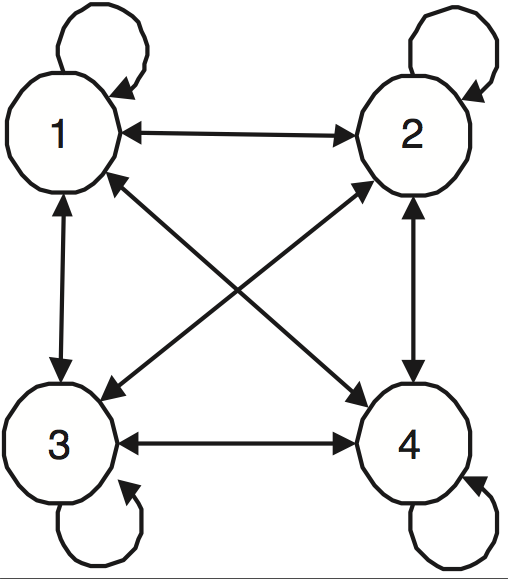
\epsfig{file=topo1, width=3cm}}\quad
        \subfloat[] {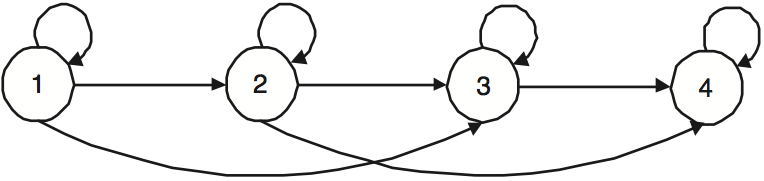
\epsfig{file=topo2, width=8cm}}
    }
    \caption{Types of HMMs: (a) Ergodic model, and (b) Left-right model}
    \label{FIG:topology-hmm}
\end{figure}


\subsection{The Three Basic Problems for HMMs}

Given a model, three basic problems of interest must be solved for the model to
be useful in real-word applications. These problems are the following:

\begin{itemize}

    \item The evaluation problem: given an observation sequence
        $O = (o_0, o_1, \ldots, o_{T-1})$, and a model $\lambda = (A, A', B, \pi)$,
        how do we compute $P(O | \lambda)$, the probability of $O$ given $\lambda$ ?

    \item The decoding problem: given the observation sequence
        $O = (o_0, o_1, \ldots, o_{T-1})$, and the model $\lambda$,
        how do we find the optimal state sequence in $\lambda$ that has generated $O$ ?

    \item The training problem: given a set of observation sequences and
        an initial model $\lambda$, how can we re-estimate the model parameters so as
        to increase the likelihood of generating this set of sequences ?

\end{itemize}


\subsubsection{The Evaluation Problem}
\label{AP:the-evalution-problem}

To compute $P(O | \lambda)$, we modify the well-known Forward-Backward
procedure \cite{Rabiner89} to take into account the assumption that symbols are
emitted along transitions, the possibility of null transitions, and the use of
multiple codebooks. Hence, we define the forward probability $\alpha_t(i)$ as:

\begin{equation}
    \alpha_t(i) = P(o_0, o_1, \ldots, o_{t-1}, q_t = s_i | \lambda)
    \label{EQ:alpha}
\end{equation}

\noindent where $\alpha_t(i)$ is the probability of the partial observation
sequence $(o_0, o_1 \ldots, o_{t-1})$ (until time $t-1$) and the state $s_i$
reached at time $t$ given the model $\lambda$. $\alpha_t(i)$ can be inductively
computed as follows.

\begin{enumerate}
\item \textit{Initialization}

\begin{equation}
    \alpha_0(0) = 1.0
    \label{EQ:alpha-initialization}
\end{equation}

$$\alpha_{0}(j) = \sum_{i=0}^{N-1} a'_{ij} \alpha_0(i) \quad j = 0, 1, \dots, N-1$$

\noindent given that $s_0$ is the only possible initial state.


\item \textit{Induction}

\begin{equation}
    \alpha_t(j) = \sum_{i=0}^{N-1} \left[ a_{ij} \left( \prod_{p=0}^{P-1} b_{ij}^p(o_{t-1}) \right)
                            \alpha_{t-1}(i) + a'_{ij} \alpha_t(i) \right] \\
    \label{EQ:alpha-induction}
\end{equation}

$$j = 0, 1, \dots, N-1 \quad and \quad t = 1, 2, \dots, T$$


\item \textit{Termination}

\begin{equation}
    P(O|\lambda) = \alpha_T(N-1)
    \label{EQ:alpha-termination}
\end{equation}
\end{enumerate}

\noindent given that $s_{N-1}$ is the only possible terminal state. Similarly,
we define the backward probability $\beta_t(i)$ by:

\begin{equation}
    \beta_t(i) = P(o_t, o_{t+1}, \ldots, o_{T-1} | q_t = s_i, \lambda)
    \label{EQ:beta}
\end{equation}

\noindent where $\beta_t(i)$ is the probability of the partial observation
sequence from the time $t$ to the end, given state $s_i$ reached at time $t$
and the model $\lambda$. $\beta_t(i)$ can also be inductively computed as
follows.

\begin{enumerate}
\item \textit{Initialization}

\begin{equation}
    \beta_T(N-1) = 1.0
    \label{EQ:beta-initialization}
\end{equation}

$$\beta_T(i) = \sum_{j=0}^{N-1} a'_{ij} \beta_T(j) \quad i = 0, 1, \dots, N-1$$

\noindent given that $s_{N-1}$ is the only possible terminal state.


\item \textit{Induction}

\begin{equation}
    \beta_{t}(i) = \sum_{j=0}^{N-1} \left[ a_{ij} \left( \prod_{p=0}^{P-1}  b_{ij}^p(o_t) \right)
                        \beta_{t+1}(j) + a'_{ij} \beta_t(j) \right]
    \label{EQ:beta-induction}
\end{equation}

$$\quad t = T-1, T-2, \ldots, 0 \quad and \quad i = 0, 1, \ldots, N-1$$


\item \textit{Termination}

\begin{equation}
    P(O|\lambda) = \beta_0(0)
    \label{EQ:beta-termination}
\end{equation}
\end{enumerate}

\noindent given that $q_0$ is the only possible initial state.


\subsubsection{The Decoding Problem}
\label{AP:the-decoding-problem}


The decoding problem is solved using a near-optimal procedure, the Viterbi
algorithm, by looking for the best state sequence $Q = (q_0, q_1, \ldots, q_T)$
for the given observation sequence $O = (o_0, o_1, \ldots, o_{T-1})$. Again, we
modify the classic algorithm \cite{Rabiner89} in the following way.

\begin{equation}
\delta_t(i) = \max_{q_0, q_1, \ldots, q_{t-1}}
    P[q_0, q_1, \ldots, q_t, q_t = s_i, o_0, o_1, \ldots, o_{t-1} | \lambda]
    \label{EQ:delta}
\end{equation}

\noindent where $\delta_t(i)$ is the probability of the best path that accounts
for the first $t$ observations and ends at state $s_i$ at time $t$. The
function $\Psi_t(i)$ is defined to recover the best state sequence by a
procedure called Backtracking. $\Psi_t(i)$ e $\delta_t(i)$ can be recursively
computed as follows.

\begin{enumerate}
\item \textit{Initialization}

\begin{equation}
    \delta_0(0) = 1.0
    \label{EQ:delta-initialization}
\end{equation}

$$\Psi_0(0) = 0$$

$$\delta_0(j) = \max_{0 \leq i \leq N-1} [ \delta_0(i) a'_{ij} ] \quad j = 0, 1, \dots, N-1$$

$$\Psi_0(j) = \arg \max_{0 \leq i \leq N-1} [ \delta_0(i) a'_{ij} ] \quad j = 0, 1, \dots, N-1$$

\noindent given that $s_0$ is the only possible initial state.


\item \textit{Recursion}

\begin{equation}
    \delta_t(j) = \max_{0 \leq i \leq N-1} \left[ a_{ij} \left( \prod_{p=0}^{P-1} b_{ij}^p(o_{t-1}) \right)
                        \delta_{t-1}(i); a'_{ij} \delta_t(i) \right]
    \label{EQ:delta-recursion}
\end{equation}

$$t = 1, 2, \ldots, T \quad and \quad j = 0, 1, \ldots, N-1$$

\begin{equation}
    \Psi_t(j) = \arg \max_{0 \leq i \leq N-1} \left[ a_{ij} \left( \prod_{p=0}^{P-1} b_{ij}^p(o_{t-1}) \right)
                        \delta_{t-1}(i); a'_{ij} \delta_t(i) \right]
    \label{EQ:psi-recursion}
\end{equation}

$$t = 1, 2, \ldots, T \quad and \quad j = 0, 1, \ldots, N-1$$


\item \textit{Termination}

\begin{equation}
    P^* = \delta_T(N-1)
    \label{EQ:delta-termination-1}
\end{equation}

\begin{equation}
    q_T^* = (N-1)
    \label{EQ:delta-termination-2}
\end{equation}

\noindent given that $s_{N-1}$ is the only possible terminal state.

\item \textit{Backtracking procedure}

\begin{equation}
    q_t^* = \Psi_{t+1} (q_{t+1}^*), \quad t=T-1, T-2, \ldots, 0
    \label{EQ:backtracking-procedure}
\end{equation}
\end{enumerate}

As shown above, except for the Backtracking procedure, Viterbi and Forward
procedures are similar. The only difference is that the summation is replaced
by maximization.


\subsubsection{The Training Problem}
\label{AP:the-training-problem}

The main strength of HMMs is the existence of a procedure called the Baum-Welch
algorithm \cite{Jelinek97,Rabiner89} that iteratively and automatically adjusts
HMM parameters given a training set of observation sequences. This algorithm,
which is an implementation of the Expectation-Maximization algorithm
\cite{Moom96}, guarantees the model to converge to a local maximum of the
probability of observation of the training set according to the maximum
likelihood estimation criterion. This maximum depends strongly on the initial
parameters.

To re-estimate HMM parameters, we first define $\xi_t^1(i,j)$, the probability
of being in state $s_i$ at time $t$ and in state $s_j$ at time $(t+1)$,
producing a real observation $O_t$, given the model and the observation $O$,
and $\xi_t^2(i,j)$, the probability of being in state $i$ at time $t$ and in
state $j$ at time $t$, producing the null observation $\Phi$, given the model
and the observation $O$.

\begin{equation}
    \xi_t^1(i,j) = P(q_t = s_i, q_{t+1} = s_j | O, \lambda)
    \label{EQ:xi-1}
\end{equation}

\begin{equation}
    \xi_t^2(i,j) = P(q_t = s_i, q_t = s_j | O, \lambda)
    \label{EQ:xi-2}
\end{equation}

The development of these quantities leads to:

\begin{equation}
    \xi_t^1(i,j) = \frac{ \alpha_t(i) a_{ij} \left( \prod_{p=0}^{P-1} b_{ij}^p(o_t) \right) \beta_{t+1}(j)} { P(O | \lambda) }
    \label{EQ:xi-3}
\end{equation}

\begin{equation}
    \xi_t^2(i,j) = \frac{ \alpha_t(i) a'_{ij} \beta_t(j)} { P(O | \lambda) }
    \label{EQ:xi-4}
\end{equation}

We also define $\gamma_t(i)$ as the probability of being in state $s_i$ at time
$t$, given the model and the observation sequence.

\begin{equation}
    \gamma_t = P(q_t = s_i | O, \lambda)
    \label{EQ:gamma-1}
\end{equation}

$\gamma_t(i)$ is related to $\xi_t^1(i,j)$ and $\xi_t^2(i,j)$ by the following
equation:

\begin{equation}
    \gamma_t =
        \sum_{j=0}^{N-1} [ \xi_t^1(i,j) + \xi_t^2(i,j) ] = \frac{\alpha_t(i) \beta_t(i)} {P(O | \lambda)}
    \label{EQ:gamma-2}
\end{equation}

The re-estimations of HMM parameters $\{ a_{ij} \}$, $\{ a'_{ij} \}$ e $\
\{b_{ij}^p(k) \}$ are:

\begin{equation}
    \overline{a_{ij}} =
        \frac{ \mbox{ \scriptsize{expected number of transitions from
                        $s_i$ at time $t$ to $s_j$ at time $(t+1)$ }}}
             { \mbox{\scriptsize{expected number of being in $s_i$ }}}
    \label{EQ:a-1}
\end{equation}

\begin{equation}
    \overline{a'_{ij}} =
        \frac{ \mbox{ \scriptsize{expected number of transitions from
                    $s_i$ at time $t$ to $s_j$ at time $t$ and observing $\Phi$ }}}
             { \mbox{ \scriptsize{expected number of being in $s_i$ }}}
    \label{EQ:a2-1}
\end{equation}

\begin{equation}
\overline{b_{ij}^p(k)} =
    \frac{ \mbox{ \scriptsize{expected number of symbols $v_k^p$ in transition
                    from $s_i$ at time $t$ to $s_j$ at time $(t+1)$ }}}
         { \mbox{ \scriptsize{expected number of transitions in $s_i$
                    at time $t$ to $s_j$ at time $(t+1)$ }}}
    \label{EQ:b-1}
\end{equation}

Given the definitions of $\xi_t^1(i,j)$, $\xi_t^2(i,j)$, and $\gamma_t(i)$, it
is easy to see, when we are using one observation sequence $O$:

\begin{equation}
    \overline{a_{ij}} =
        \frac{ \sum_{t=0}^{T-1} \xi_t^1(i,j) } { \sum_{t=0}^T \gamma_t(i) } =
        \frac{ \sum_{t=0}^{T-1} \alpha_t(i) a_{ij} \left( \prod_{p=0}^{P-1} b_{ij}^p(o_t) \right) \beta_{t+1}(j) }
             { \sum_{t=0}^T \alpha_t(i) \beta_t(i) }
     \label{EQ:a-2}
\end{equation}

\begin{equation}
    \overline{a'_{ij}} =
        \frac{ \sum_{t=0}^{T-1} \xi_t^2(i,j) } { \sum_{t=0}^T \gamma_t(i) } =
        \frac{ \sum_{t=0}^{T-1} \alpha_t(i) a'_{ij} \beta_t(j) }
            { \sum_{t=0}^T \alpha_t(i) \beta_t(i) }
    \label{EQ:a2-2}
\end{equation}

\begin{equation}
    \overline{b_{ij}^p(k)} =
        \frac{ \sum_{t=0}^{T-1} \delta(o_t^p, v_k^p) \xi_t^1(i,j) }
             { \sum_{t=0}^{T-1} \xi_t^1(i,j) } =
        \frac{ \sum_{t=0}^{T-1} \delta(o_t^p, v_k^p) \alpha_t(i) a_{ij} \left( \prod_{p=0}^{P-1} b_{ij}^p(o_t) \right) \beta_{t+1}(j) }
             { \sum_{t=0}^{T-1} \alpha_t(i) a_{ij} \left( \prod_{p=0}^{P-1} b_{ij}^p(o_t) \right) \beta_{t+1}(j) }
    \label{EQ:b-2}
\end{equation}

\noindent where $\delta(x,y) = \left ( \begin{array} {cc}
                    1 & \quad if x = y \\
                    0 & \quad if x \ne y
                \end{array}\right)$

For a set of training sequences $O(0), O(1), \ldots, O(U-1)$ (size $U$), as is
usually the case in real world applications, the above formulas become:

\begin{equation}
    \overline{a_{ij}} =
        \frac{ \sum_{u=0}^{U-1} \sum_{t=0}^{T-1} \xi_t^1(i,j,u)}
             { \sum_{u=0}^{U-1} \sum_{t=0}^T \gamma_t(i,u)} =
        \frac{ \sum_{u=0}^{U-1} \frac{1} {P(u)} \sum_{t=0}^{T-1}
               \alpha_t(i,u) a_{ij} \left( \prod_{p=0}^{P-1} b_{ij}^p(o_t^p(u)) \right) \beta_{t+1}(j,u) }
             { \sum_{u=0}^{U-1} \frac{1} {P(u)} \sum_{t=0}^T \alpha_t(i,u) \beta_t(i,u) }
    \label{EQ:a-3}
\end{equation}

\begin{equation}
    \overline{a'_{ij}} =
        \frac{ \sum_{u=0}^{U-1} \sum_{t=0}^{T-1} \xi_t^2(i,j,u) }
             { \sum_{u=0}^{U-1} \sum_{t=0}^T \gamma_t(i,u)} =
        \frac{ \sum_{u=0}^{U-1} \frac{1} {P(u)} \sum_{t=0}^{T-1} \alpha_t(i,u) a'_{ij} \beta_t(j,u) }
             { \sum_{u=0}^{U-1} \frac{1} {P(u)} \sum_{t=0}^T \alpha_t(i,u) \beta_t(i,u) }
    \label{EQ:a2-3}
\end{equation}

\begin{equation}
    \overline{b_{ij}^p(k)} =
        \frac{ \sum_{u=0}^{U-1} \sum_{t=0}^{T-1} \delta(o_t^p(u), v_k^p) \xi_t^1(i,j,u) }
             { \sum_{u=0}^{U-1} \sum_{t=0}^{T-1} \xi_t^1(i,j,u)}
    \label{EQ:b-3}
\end{equation}

$$\overline{b_{ij}^p(k)} =
    \frac{ \sum_{u=0}^{U-1} \frac{1} {P(u)} \sum_{t=0}^{T-1} \delta(o_t^p(u), v_k^p)
                       \alpha_t(i,u) a_{ij} \left( \prod_{p=0}^{P-1} b_{ij}^p(o_t^p(u)) \right) \beta_{t+1}(j,u) }
         { \sum_{u=0}^{U-1} \frac{1} {P(u)} \sum_{t=0}^{T-1}
                       \alpha_t(i,u) a_{ij} \left( \prod_{p=0}^{P-1} b_{ij}^p(o_t^p(u)) \right) \beta_{t+1}(j,u)}$$

In the above equations, the index $u$ is introduced into $\alpha$, $\beta$,
$\xi^1$, $\xi^2$, and $\gamma$ to indicate the observation sequence $O(u)$
currently used. Note that a new quantity $P(u) = P(O(u) | \lambda)$ appears,
since this term is now included in the summation and cannot be eliminated as
before.

If we define the current model as $\lambda = (A, A', B_p, \pi)$ and the
re-estimated model as $\overline{\lambda} = ( \overline{A}, \overline{A'},
\overline{B_p}, \overline{\pi})$, and we iteratively use $\overline{\lambda}$
in place of $\lambda$ and repeat the re-estimation calculation, we can then
improve the probability of $O$ being observed from the model until some
limiting point is reached. The final result of this re-estimation procedure is
a maximum likelihood estimate of the HMM. It should be pointed out that the
Forward-Backward algorithm leads to a local maxima only, and that in most
problems of interest, the likelihood function is very complex and has many
local maxima.

\section{Modelling Handwritten Words using HMMs}
\label{modelling:Sec}

Based on our previous experience, we decided to represent the characters using the maximum of three graphemes. In light of this, four states are necessary for each character model as depicted in Figure \ref{charactermodel:fig}. This model is based on the architecture proposed by El Yacoubi et al \cite{El99}.

\begin{figure}[htbp]
   \centering
   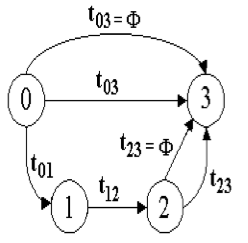
\epsfig{file=charactermodel, width=4cm}
   \caption{Character model architecture}
   \label{charactermodel:fig}
\end{figure}


In this model, the observation sequences are emitted from the model transitions in order to take advantage of the explicit segmentation adopted during feature extraction. All possible segmentation outcomings are reported in Table \ref{seg-outcoming:tab}. Considering the database we are using for the experiments so far, the month alphabet is composed of 20-character classes, therefore,we have 40 HMMs considering uppercase and lowercase characters.


\begin{table} [ht!]
\caption {Transitions allowed by the character model}
\begin{center}
\begin{tabular}{ll} \hline 
 \multicolumn{1}{c}{Transition}&
 \multicolumn{1}{c}{Description} \\ \hline

$t_{03} = \Phi $ & character under-segmentation \\
$t_{03}$         & no segmentation detected \\
$t_{01}-t_{12}-(t_{23} = \Phi)$ & character over-segmented into 2 graphemes \\
$t_{01}-t_{12}-t_{23}$ & character over-segmented into 3 graphemes \\ \hline


\end{tabular}
\label{seg-outcoming:tab}
\end{center}
\end{table}

\subsection{Training the Models}

Since the writing style (uppercase/lowercase) of each training word image is available, the word model is generated from the concatenation of appropriate character models. The last state of a character model becomes the initial state of the next model, as depicted in Figure \ref{training-model:fig}.

\begin{figure}[htbp]
   \centering
   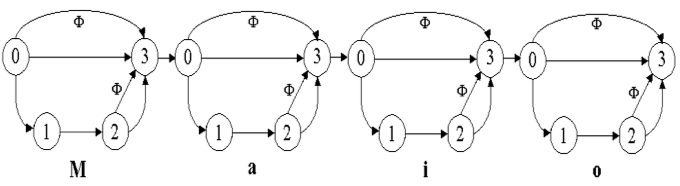
\epsfig{file=trainingmodel, width=10cm}
   \caption{Training model of class ``Maio''}
   \label{training-model:fig}
\end{figure}
 
In order to train the models, we are using the Baum-Welch algorithm (described in Section \ref{AP:the-training-problem}) with cross-validation procedure. The program used to train the HMM models is available in the following directory:

\begin{verbatim}
~/tools/orand/batch/crossv
\end{verbatim}

To execute the training, use:
\begin{verbatim}
./orand_crossanmt feat1 ex01 symbol_1.ex01 m_month.ex01
\end{verbatim}
 
\subsection{Recognition}

Since we are dealing with unconstrained handwriting, one can write the month using uppercase, lowercase, or a mix of both. With this in mind, we have used three different HMM configurations for recognition. The programs used for recognition are available in the following directory:

\begin{verbatim}
~/tools/orand/batch/rec/an
\end{verbatim}


First we have built 24 models (similar to the one presented in Figure \ref{training-model:fig}), 12 for lowercase and 12 for uppercase. To recognise using 24 models, use:
\begin{verbatim}
./orand_recanmt24cb 1 feat1 ex01 symbol_1.ex01 m_month.ex01
\end{verbatim}

In the second experiment, we have added another 12 models, summing up 36 models, where the first letter is uppercase and all the others lowercase. To recognise using 36 models, use:
\begin{verbatim}
./orand_recanmt36cb 1 feat1 ex01 symbol_1.ex01 m_month.ex01
\end{verbatim}

However, none of these strategies are able to handle the problem of mixed handwriting styles. To deal with that, the third model, inspired in the work of El Yacoubi \cite{El99}, is composed of two character models in parallel (uppercase and lowercase), as depicted in Figure \ref{paralel-models:fig}.

\begin{figure}[htbp]
   \centering
   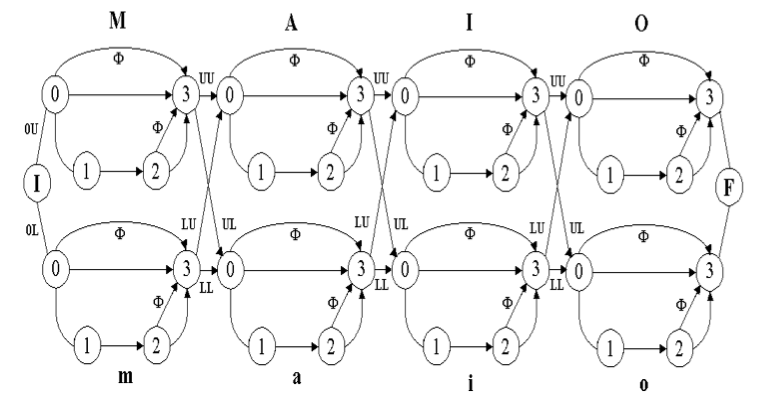
\epsfig{file=paralel-models, width=14cm}
   \caption{Training model of class ``Maio''}
   \label{paralel-models:fig}
\end{figure}
 
The word model consists of an initial state (I) and a final state (F), and two consecutive character models linked by four transitions: two uppercase characters (UU), two lowercase characters (LL), one uppercase character followed by one lowercase character (UL) and one lowercase character followed by one uppercase character (LU). The probabilities of these transitions are estimated by their occurrence frequency in the training set. In the same manner, the probabilities of beginning a word by an uppercase character (0U) or lowercase character (0L) are also estimated. This architecture handles the problem related to the mixed handwritten words detecting implicitly the writing style during recognition using the Backtracking procedure of the Viterbi algorithm. To recognise using 12 models (in parallel), use:
\begin{verbatim}
- /orand_recanmt12 1 feat1 ex01 symbol_1.ex01 m_month.ex01
\end{verbatim}


\section{Experiments}
\label{experiments:sec}
In these experiments we have used the Brazilian month word database, which is composed of 2,000 images. It was divided into 1,190, 408 and 400 images for training, validation, and testing, respectively. The results reported in this section were carried out on the test using the Forward procedure. Table \ref{results:tab} summarises the results of the three experiments using the Global features (20 components).



\begin{table} [ht!]
\caption {Summary of the recognition rates obtained in the experiments}
\begin{center}
\begin{tabular}{ccc} \hline 
 \multicolumn{1}{c}{Experiment}&
 \multicolumn{1}{c}{Number of HMM Models} &
 \multicolumn{1}{c}{Rec. Rate (\%)} \\ \hline

I & 24 & 80.9 \\
II & 36 & 82.2 \\
III & 12 & 82.4 \\ \hline


\end{tabular}
\label{results:tab}
\end{center}
\end{table}

As one can notice, the third model achieve a slightly better result with a considerable smaller number of HMM models. These results show that the parallel model can handle better the mixture of handwriting styles. In spite of the similar results, by analysing the confusion matrices (Tables \ref{cmI:tab}, \ref{cmII:tab}, and \ref{cmIII:tab} ), one can notice that in some cases the three models make different mistakes. This suggests that this kind of complementarity may be explored by fusing the three different strategies in order to increase the recognition rates. This will be subject of further investigation during the project.

\begin{table} [ht!]
\caption {Confusion Matrix (\%) - Experiment I}
\begin{center}
\begin{tabular}{rrrrrrrrrrrrr} \hline 
 \multicolumn{1}{c}{Class}&
 \multicolumn{1}{c}{1}&
 \multicolumn{1}{c}{2}&
 \multicolumn{1}{c}{3}&
 \multicolumn{1}{c}{4}&
 \multicolumn{1}{c}{5}&
 \multicolumn{1}{c}{6}&
 \multicolumn{1}{c}{7}&
 \multicolumn{1}{c}{8}&
 \multicolumn{1}{c}{9}&
 \multicolumn{1}{c}{10}&
 \multicolumn{1}{c}{11}&
 \multicolumn{1}{c}{12} \\ \hline


1 &	 \textbf{73.7} &	 10.5 	& 5.3 	& -   	& -   	& 5.3 	& 2.6 	& -   	& 2.6 	& -   	& -   	& -   \\
2 &	 3.1 &	 \textbf{84.4} 	& 6.3 	& -   	& -   	& -   	& -   	& -   	& -   	& 3.1 	& 3.1 	& -   \\
3 &	 -   &	 2.8 	& \textbf{69.4} 	& 2.8 	& 25.0 	& -   	& -   	& -   	& -   	& -   	& -   	& -   \\
4 &	 -  & 	 -   	& -   	& \textbf{82.1} 	& 12.8 	& -   	& -   	& 2.6 	& 2.6 	& -   	& -   	& -   \\
5 &	 -   &	 2.6 	& -   	& 5.3 	& \textbf{86.8} 	& -   	& -   	& 5.3 	& -   	& -   	& -   	& -   \\
6 &	 3.4 &	 -   	& -   	& -   	& 3.4 	& \textbf{89.7} 	& -   	& -   	& 3.4 	& -   	& -   	& -   \\
7 &	 3.1 &	 -   	& 3.1 	& -   	& 6.3 	& 12.5 	& \textbf{75.0} 	& -   	& -   	& -   	& -   	& -   \\
8 &	 -   &	 -   	& 3.6 	& -   	& 7.1 	& -   	& -   	& \textbf{82.1} 	& -   	& -   	& -   	& 7.1 \\
9 &	 3.2 &	 -   	& -   	& -   	& -   	& -   	& -   	& -   	& \textbf{83.9} 	& 9.7 	& -   	& 3.2 \\
10&	 -   &	 -   	& -   	& -   	& -   	& -   	& -   	& -   	& 13.3 	& \textbf{86.7} 	& -   	& -   \\
11&	 2.9 &	 -   	& -   	& -   	& -   	& -   	& -   	& -   	& 5.9 	& 2.9 	& \textbf{88.2} 	& -  \\ 
12&	 -   &	 -   	& -   	& -   	& -   	& -   	& -   	& 6.1 	& 15.2 	& 9.1 	& -   	& \textbf{69.7}\\ \hline 

\end{tabular}
\label{cmI:tab}
\end{center}
\end{table}



\begin{table} [ht!]
\caption {Confusion Matrix (\%) - Experiment II}
\begin{center}
\begin{tabular}{rrrrrrrrrrrrr} \hline 
 \multicolumn{1}{c}{Class}&
 \multicolumn{1}{c}{1}&
 \multicolumn{1}{c}{2}&
 \multicolumn{1}{c}{3}&
 \multicolumn{1}{c}{4}&
 \multicolumn{1}{c}{5}&
 \multicolumn{1}{c}{6}&
 \multicolumn{1}{c}{7}&
 \multicolumn{1}{c}{8}&
 \multicolumn{1}{c}{9}&
 \multicolumn{1}{c}{10}&
 \multicolumn{1}{c}{11}&
 \multicolumn{1}{c}{12} \\ \hline
 
1	& \textbf{76.3} 	& 7.9 	& 5.3 	& -   	& -   	& 5.3 	& 2.6 	& -   	& 2.6 	& -   	& -   	& -   \\
2	& 3.1 	& \textbf{90.6} 	& 3.1 	& -   	& -   	& -   	& -   	& -   	& -   	& 3.1 	& -   	& -   \\
3	& -   	& 2.8 	& \textbf{66.7} 	& 2.8 	& 27.8 	& -   	& -   	& -   	& -   	& -   	& -   	& -   \\
4	& 2.6 	& -   	& -   	& \textbf{84.6} 	& 12.8 	& -   	& -   	& -   	& -   	& -   	& -   	& -   \\
5	& -   	& -   	& -   	& 10.5 	& \textbf{86.8} 	& -   	& -   	& 2.6 	& -   	& -   	& -   	& -   \\
6	& 3.4 	& -   	& -   	& -   	& 3.4 	& \textbf{93.1} 	& -   	& -   	& -   	& -   	& -   	& -   \\
7	& 3.1 	& -   	& 6.3 	& -   	& 3.1 	& 12.5 	& \textbf{71.9} 	& 3.1 	& -   	& -   	& -   	& -   \\
8	& -   	& -   	& 3.6 	& -   	& 7.1 	& -   	& -   	& \textbf{85.7} 	& -   	& -   	& -   	& 3.6 \\
9	& 3.2 	& -   	& -   	& -   	& -   	& -   	& -   	& -   	& \textbf{83.9} 	& 9.7 	& -   	& 3.2 \\
10	& -   	& -   	& -   	& -   	& -   	& -   	& -   	& -   	& 16.7 	& \textbf{83.3} 	& -   	& -   \\
11	& -   	& 2.9 	& -   	& -   	& -   	& -   	& -   	& -   	& 2.9 	& 2.9 	& \textbf{91.2} 	& -   \\
12	& -   	& -   	& -   	& -   	& -   	& -   	& -   	& 3.0 	& 12.1 	& 9.1 	& 3.0 	& \textbf{72.7} \\ \hline

\end{tabular}
\label{cmII:tab}
\end{center}
\end{table}




\begin{table} [ht!]
\caption {Confusion Matrix (\%) - Experiment III}
\begin{center}
\begin{tabular}{rrrrrrrrrrrrr} \hline 
 \multicolumn{1}{c}{Class}&
 \multicolumn{1}{c}{1}&
 \multicolumn{1}{c}{2}&
 \multicolumn{1}{c}{3}&
 \multicolumn{1}{c}{4}&
 \multicolumn{1}{c}{5}&
 \multicolumn{1}{c}{6}&
 \multicolumn{1}{c}{7}&
 \multicolumn{1}{c}{8}&
 \multicolumn{1}{c}{9}&
 \multicolumn{1}{c}{10}&
 \multicolumn{1}{c}{11}&
 \multicolumn{1}{c}{12} \\ \hline

1 & \textbf{73.6} 	& 7.8 	& 5.2 	& -   	& -   	& 2.6 	& 2.6 	& -   	& 5.2 	& 2.6 	& -   	& -   \\
2 & 3.1 	& \textbf{84.3} 	& 3.1 	& -   	& -   	& -   	& -   	& -   	& 3.1 	& 3.1 	& 3.1	& -   \\
3 & -   	& 2.7 	& \textbf{66.6} 	& 2.78 	& 27.7 	& -   	& -   	& -   	& -   	& -   	& -   	& -   \\
4 & -   	& -   	& -   	& \textbf{89.7} 	& 10.2 	& -   	& -   	& -   	& -   	& -   	& -   	& -   \\
5 & -   	& -   	& -   	& 7.8 	& \textbf{86.8} 	& -   	& -   	& 2.6 	& 2.6 	& -   	& -   	& -   \\
6 & 3.4 	& -   	& -   	& -   	& 3.4 	& \textbf{93.1} 	& -   	& -   	& -   	& -   	& -   	& -   \\
7 & 3.1 	& -   	& 6.2 	& -   	& 3.1 	& 12.5 	& \textbf{71.8} 	& 3.1 	& -   	& -   	& -   	& -   \\
8 & -   	& -   	& 3.5 	& -   	& 7.1 	& -   	& -   	& \textbf{85.7} 	& -   	& -   	& -   	& 3.5 \\
9 & 3.2 	& -   	& -   	& -   	& -   	& -   	& -   	& -   	& \textbf{83.8} 	& 6.4 	& -   	& 6.4 \\
10&  -   & -   	& -   	& -   	& -   	& -   	& -   	& -   	& 16.6 	& \textbf{83.3} 	& -   	& -   \\
11&  -   & -   	& -   	& -   	& -   	& -   	& -   	& -   	& 2.9 	& 2.9 	& \textbf{94.1} 	& -   \\
12&  -   & -   	& -   	& -   	& -   	& -   	& -   	& 3.0 	& 12.1 	& 9.0 	& -   	& \textbf{75.7} \\ \hline

\end{tabular}
\label{cmIII:tab}
\end{center}
\end{table}

Another aspect worth of noticing is the TOP3 result for the model used in the third experiment. In this case, considering TOP3 (Table \ref{cmIIITOP2:tab}), the classifier would produce a recognition rate of 96.4\%. This result indicates that a verification strategy would be a possible alternative to recover some of these confusions. This subject also will be investigated in this project.


\begin{table} [ht!]
\caption {Confusion Matrix (\%) - TOP3 for Experiment III}
\begin{center}
\begin{tabular}{rrrrrrrrrrrrr} \hline 
 \multicolumn{1}{c}{Class}&
 \multicolumn{1}{c}{1}&
 \multicolumn{1}{c}{2}&
 \multicolumn{1}{c}{3}&
 \multicolumn{1}{c}{4}&
 \multicolumn{1}{c}{5}&
 \multicolumn{1}{c}{6}&
 \multicolumn{1}{c}{7}&
 \multicolumn{1}{c}{8}&
 \multicolumn{1}{c}{9}&
 \multicolumn{1}{c}{10}&
 \multicolumn{1}{c}{11}&
 \multicolumn{1}{c}{12} \\ \hline

1	& \textbf{92.1} 	& -   	& 2.6 	&    - &  	 -  & 	 2.6& 	 -  & 	 - &  	 -  & 	 2.6 &	 -  & 	 - \\  
2	& -   	& \textbf{96.8} 	& -   	&    - &  	 -  & 	 -  & 	 -  & 	 - &  	 -  & 	 3.1 & 	 -  & 	 -  \\ 
3	& -   	& -   	& \textbf{100.0} &	 - &  	 -  & 	 -  & 	 -  & 	 - &  	 -  & 	 -   &	 -  & 	 -  \\ 
4	& -   	& -   	& -   	& \textbf{92.3} &	 7.6 	& -   	& -   	& -   &	 -   	& -   	 &-   	& -   \\
5	& -   	& -   	& -   	& 2.6 	& \textbf{92.1} 	& -   	& -   	& 2.6 &	 2.6 	 &-   	 &-   	& -   \\
6	& -   	& -   	& -   	& -   	& 3.4 	& \textbf{96.5} 	& -   	& -   &	 -   	& -   	 &-   	& -   \\
7	& 3.1 	& -   	& -   	& -   	& -   	& -   	& \textbf{96.8} 	& -   	& -   	& -   	 &-   	& -   \\
8	& -   	& -   	& -   	& -   	& -   	& -   	& -   	& \textbf{100.0}& 	 -  & 	 -   &	 -  & 	 -  \\ 
9	& 3.2 	& -   	& -   	& -   	& -   	& -   	& -   	& -   	& \textbf{96.7} 	& -   	 &-   	 &-   \\
10	& -   	& -   	& -   	& -   	& -   	& -   	& -   	& -   	& 3.3 	& \textbf{96.6} 	 &-   	 &-   \\
11	& -   	& -   	& -   	& -   	& -   	& -   	& -   	& -   	& -   	& -   	 &\textbf{100.0} &	 -  \\ 
12	& -   	& -   	& -   	& -   	& -   	& -   	& -   	& -   	& 3.0 	& -   	 &-   	 &\textbf{96.9} \\ \hline

\end{tabular}
\label{cmIIITOP2:tab}
\end{center}
\end{table}



\section{Conclusions}
\label{conclusion:sec}

In this report we have summarised the results of the experiments using the global features to train the HMM models to recognise unconstrained handwritten month words. These results show that the parallel model seems to be a good alternative for our application providing a recognition rate of 82.5\% and 96.4\% for TOP1 and TOP3, respectively. Our next steps will be towards the combination of different architectures of HMMs and the implementation of a different feature set, which is based on concavities. 



\bibliographystyle{IEEEbib}
\bibliography{refer}



\end{document}



